\question{Ядерная модель атома и опыты Резерфорда. Теория рассеяния 
альфа-частиц. Дифференциальное эффективное сечение рассеяния.}

О том, как распределяются положительный и отрицательные заряды в атоме можно
выяснить, произведя непосредственное зондирование внутренней области атомов.
Такой опыт осуществил Резерфорд в 1911 году изучая изменение направления
\( \alpha \)-частиц при их прохождении через тонкие слои вещества.

\begin{minipage}{.4\textwidth}
    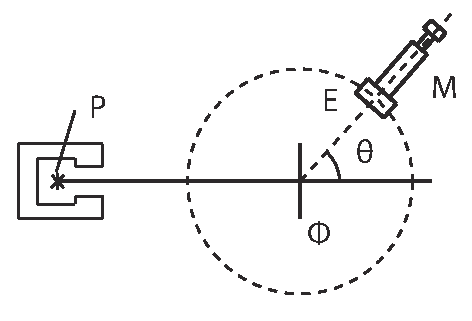
\includegraphics[width=\textwidth]{03_install}
\end{minipage}
\begin{minipage}{.55\textwidth}
    Узкое отверстие формирует узкий пучок \( \alpha \)-частиц, испускаемых
    радиоактивным веществом \emph{РВ}. Пучок попадает на фольгу \emph{Ф}. При
    прохождении через фольгу \( \alpha \)-частицы отклонялись на различные углы
    и попадали на экран \emph{Э} вызывая сцинтилляции (вспышки света), которые
    наблюдались в микроскоп \emph{М}. Микроскоп можно было вращать и наблюдать
    вспышки под различными углами \( \theta \). Вся установка была помещена в
    вакуум, чтобы избежать рассеяние \( \alpha \)-частиц на молекулах воздуха.
\end{minipage}

В ходе эксперимента было выяснено, что некоторые частицы отклонялись на углы
порядка \( 180^\circ \). Такое возможно, если внутри атома имеется очень сильное
электрическое поле, которое создается зарядом большой массы, сосредоточенной в
очень малом объеме. Так возникла ядерная модель Резерфорда: атом являет собой
ядро -- положительную частицу большой массы радиусом порядка \( 10^{-14} \)~м,
вокруг которого вращаются электроны.

\begin{minipage}{.4\textwidth}
    \center
    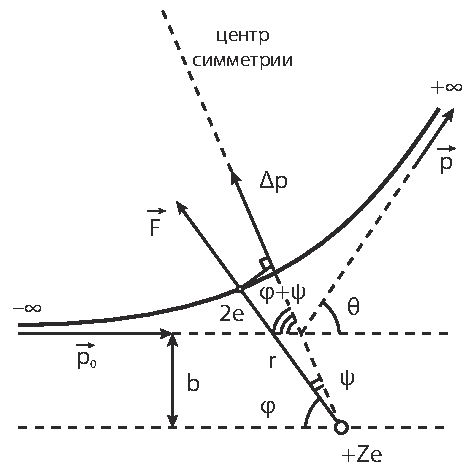
\includegraphics[width=\textwidth]{03_scheme}
    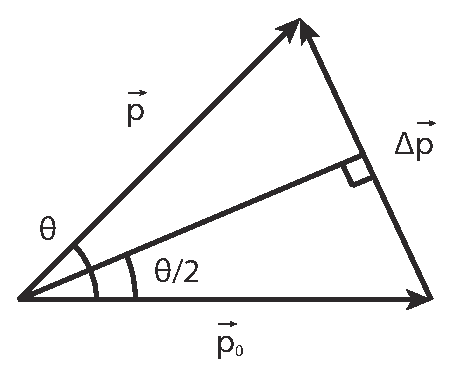
\includegraphics[width=.8\textwidth]{03_triangle}
\end{minipage}
\begin{minipage}{.55\textwidth}
    Резерфорд считал, что между ядром и \( \alpha \)-частицами действует только
    кулоновские силы, а само ядро неподвижно: \( \ds F = k\frac{2Ze^2}{r^2} \).

    Между углами существует соотношение: \( 2(\phi + \psi) = \pi - \theta \).

    Воспользуемся законом сохранения энергии, записанным для частицы на
    расстоянии \( -\infty \) и \( \infty \) от ядра, то есть до и после
    взаимодействия. Так как потенциальная энергия равна нулю, то
    \( |\vec{p}_0| = |\vec{p}| \). Изменение импульса произойдет по направлению:
    \( |\Delta\vec{p}| = 2p_0\sin\theta/2 \).
 
    Второй закон Ньютона в обобщенной формулировке:
   \[
        \vec{F} = \der{\vec{p}}{t}, \text{ откуда } d\vec{p} = \vec{F}\,dt
        \text{ и } \Delta\vec{p} = \int\vec{F}\,dt.
    \]
    В проекции:
    \[ 
        \Delta p = \int F_{\Delta p}\,dt = F\cos\psi.
    \]
\end{minipage}

Поскольку между ядром и \( \alpha \)-частицей действуют центральные силы, то
справедливы законы сохранения энергии и момента импульса.
 
Будем считать часть траектории движения \( \alpha \)-частицы как часть
окружности. Тогда:
\[
    m vb = m r^2\dot{\phi}, \quad \dot{\phi} = \der{\phi}{t} =
    \frac{vb}{r^2}, \quad dt = \frac{r^2\d\phi}{vb}.
\]
Изменение импульса:
\begin{gather*}
    \Delta p = \int F\cos\psi\cdot\frac{r^2\d\phi}{vb} = \int k\frac{2Ze^2}{r^2}
    \frac{r^2\d\phi}{vb}\cos\psi = k\frac{2Ze^2}{vb}\int\limits_0^{\pi - \theta}
    \cos\left( \frac{\pi}{2} - \frac{\theta}{2} - \phi \right)\d\phi = \\
    = k\frac{2Ze^2}{vb}\int\limits_0^{\pi - \theta} \sin\left( \phi +
    \frac{\theta}{2}\right)\d\phi = k\frac{2Ze^2}{vb}\cdot2\cos\frac{\theta}{2}.
\end{gather*}

Получаем: \( \ds 2p_0\sin\frac{\theta}{2} = k\frac{4Ze^2}{vb}\cos\frac{\theta}
{2}. \)

Начальный импульс \( \alpha \)-частицы: \( p_0 = mv \). Окончательно имеем:
\begin{equation}
    \ctg\frac{\theta}{2} = \frac{mv^2b}{2ke^2Z}.
    \label{eq:3_1}
\end{equation}

\subquestion{Дифференциальное эффективное сечение рассеяния}

\begin{minipage}{.35\textwidth}
    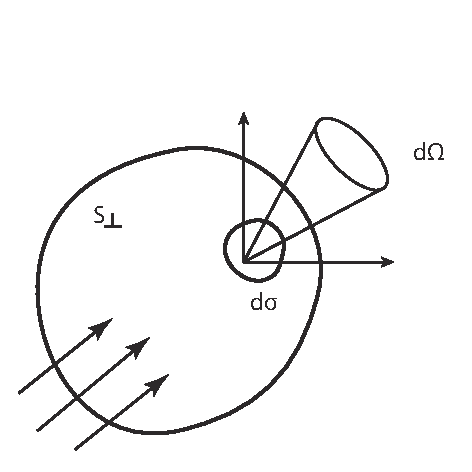
\includegraphics[width=.9\textwidth]{03_dn1}
\end{minipage}
\begin{minipage}{.6\textwidth}
Рассмотрим рассеяние потока частиц на ядре. Интенсивностью потока частиц
называют количество частиц, которые в единицу времени пересекают единичную
площадку перпендикулярно потоку: \( I = N/(\Delta t\Delta S) \).
 
При рассеянии \( dN_1 = I\d\sigma \) частиц попадают внутрь элементарного
телесного угла \( d\Omega \), величина и направление которого определяется
положением элементарной площадки \( d\sigma \).
\end{minipage}

\begin{minipage}{.55\textwidth}
Дифференциальное эффективное сечение рассеяния -- это отношение числа частиц,
рассеянных атомом в единицу времени в телесный угол \( d\Omega \), к
интенсивности падающих частиц: \( d\sigma = dN_1/I \).

Из рисунка: \( d\sigma = 2\pi b\,db \). Телесный угол, по определению:
\( d\Omega = dS/R^2 = 2\pi\sin\theta\d\theta \).

Возьмем производную от \eqref{eq:3_1}:
\[
    -\frac{1}{\sin^2\frac{\theta}{2}}\frac{d\theta}{2} = \frac{mv^2}{2kZe^2}\,db.
\]
\end{minipage}
\begin{minipage}{.4\textwidth}
    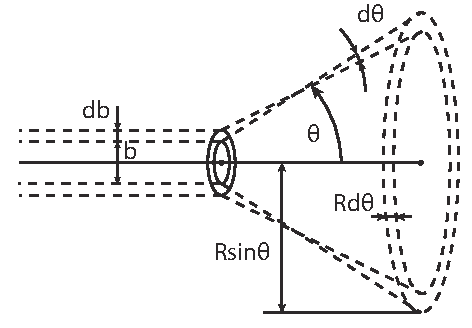
\includegraphics[width=\textwidth]{03_diff}
\end{minipage}
Тогда:
\[
    d\sigma = 2\pi\frac{2kZe^2}{mv^2}\frac{\cos\frac{\theta}{2}}{\sin\frac
    {\theta}{2}}\frac{2kZe^2}{mv^2}\frac{d\theta}{2\sin^2\frac{\theta}{2}} =
    \left( \frac{2kZe^2}{mv^2} \right)^2 \frac{2\pi\cos\frac{\theta}{2}\sin
    \frac{\theta}{2}}{2\sin^4\frac{\theta}{2}}\d\theta = \left( \frac{kZe^2}
    {mv^2} \right)^2 \frac{d\Omega}{\sin^4\frac{\theta}{2}}.
\]

Это выражение называется формулой Резерфорда для дифференциального эффективного
сечения рассеивания.

\newpage
